\chapter{Introduction to Elliptic Curves}
\section{Mathematical Foundations}
\subsection{Finite Groups}
A Finite Group is a set G with a finite number of $q$ elements, which has a binary operation $*$ : $G x G \rightarrow G$ and satisfies the following properties \cite{hankerson2006guide}:
\begin{enumerate}
	\item Associativity: $(a*b)*c=a*(b*c)$ for all elements $a,b,c \in G$
	\item Existence of an identity: there exists an element $e \in G$ such that $a*e=e*a=a$ for all $a \in G$. Element $e$ is called the identity of the group.
	\item Existence of inverses: for each element $a \in G$, there exists an element $b \in G$ such that $a*b=b*a=e$. Element $b$ is called the inverse of $a$.
\end{enumerate}
$q$ is called the group order. In addition, a group is called abelian group if it satisfies the commutativity law which is $a*b=b*a$ for all elements $a,b \in G$. 

If the binary operation is called addition (+), then the group is additive. In this case, the identity element is usually denoted by 0 and the additive inverse of an element $a$ is denoted by $-a$. If the binary operation is called multiplication $(\cdot)$, then the finite group is multiplicative. In this case, the identity element is usually denoted by 1 and the multiplicative inverse of an element $a$ is denoted by $a^{-1}$.

\subsection{Finite Fields}
Abstractly, a finite field consists of a finite set of objects called field elements together with the description of two operations, addition and multiplication, that can be performed on pairs of field elements. These operations must have certain properties \cite{hankerson2006guide}
\begin{enumerate}
	\item $(\mathbb{F},+)$ is an abelian group with (additive) identity denoted by 0.
	\item $(\mathbb{F},\cdot)$ is an abelian group with (multiplicative) identity denoted by 1.
	\item The distributive law holds: $(a+b) \cdot c = a \cdot c + b \cdot c$ for all $a,b,c \in \mathbb{F}$. 
\end{enumerate}

\paragraph{Prime Fields}\mbox{}\\
Let $p$ be a prime number. The integers modulo $p$, consisting of the integers $\left\lbrace 0,1,2,\dots,p-1\right\rbrace $ with addition and multiplication performed modulo $p$, is a finite field of order $p$.
\paragraph{Binary Fields}\mbox{}\\
Finite fields of order $2^m$ are called binary fields or characteristic-two finite fields. One way to construct $\mathbb{F}_{2^m}$ is to use a polynomial basis representation. The elements of $\mathbb{F}_{2^m}$ are the binary polynomials (polynomials whose coefficients are in the field $\mathbb{F}={0,1}$) of degree at most m-1:
$$\mathbb{F}_{2^m}=\left\lbrace a_{m-1}z^{m-1}+a_{m-2}z^{m-2}+\dots+a_2z^2+a_1z^1+a_0 : a_i \in  \left\lbrace 0,1\right\rbrace \right\rbrace $$.

An irreducible binary polynomial $f(z)$ of degree m is chosen. Irreducibility of $f(z)$ means that $f(z)$ cannot be factored as a product of binary polynomials each of degree less than $m$. Addition of field elements is the usual addition of polynomials, with coefficient performed modulo 2. Multiplication of field elements is performed modulo the reduction polynomial $f(z)$. 
\subsection{Cyclic Groups}
Let $G$ be a finite group of order $n$ with multiplication ($\cdot$) as binary operation, then $G$ is called cyclic if there exist a $g$ be an element of $G$ such that $\langle g \rangle = \left\lbrace g^i : 0 \leq i \leq r-1 \right\rbrace $ is the subgroup of $G$ generated by $g$, where $r$ is the order of the element $g$, that is, $r$ is the smallest positive integer for which $g^r = 1$. If $r=n$ then $G$ is a cyclic group with generator $g$ if $G = \langle g \rangle$. The set $\langle
 g \rangle$ is also a group itself under the same binary operation and is called the cyclic subgroup of $G$ generated by $g$.
 
%\subsection{Generalized discrete logarithm problem}
%Given a multiplicative cyclic group $(G,\cdot)$ of order n with generator g and an element $y \in \

\section{Elliptic Curves} \label{sec:EC}
An elliptic curve over a field $K$ is defined by the following equation (also known as Weierstrass from)
\begin{equation} \label{eq:ECWeierstrass}
y^3+a_1xy+a_3y = x^3 + a_2x^2+a_4x+a6
\end{equation}

where: $a_1,a_2,a_3,a_4,a_6 \in K$, and the discriminant 
 $$\Delta=-d^{2}_{2}d_{8}-8d_{4}^{3}-27d_{6}^{2}+9d_{2}d_{4}d_{6} \neq 0$$
where  
$$d_{2}=a_{1}^{2}+4a_{2}$$  $$d_{4}=2a_{4}+a_1a_3$$  $$d_6=a_{3}^{2}+4a_6$$  $$d_8=a_{1}^{2}a_6+4a_2a_6-a_1a_3a_4+a_2a_{3}^{2}-a_{4}^{2}$$

The condition $\Delta \neq 0$ guarantees that there does not exist more than one tangent line for a given point on the curve.

For an elliptic curve over a field K of characteristic $\neq$ 2 or 3, without loss of generality, we can assume that $a_1=a_2=a_3=0$, we have $d_2=0$, $d_4=2a_4$, $d_6 = 4a_6$ and $d_8=-a_{4}^{2}$. According to equation, the condition $\Delta = -16(4a_4^3+27a_6^2) \neq 0$ can be simplified to $4a_4^3+27a_6^2 \neq 0$. The curve equation is normally written is the following form:

\begin{equation} \label{eq:ECFp}
y^3=x^3+ax+b
\end{equation}

where $a=a_4$ and $b=a_6$.

For an elliptic curve over binary fields $\mathbb{F}_2^m$, without loss of generality, we can assume that $a_1=1$, $a_3=a_4=0$. Then we have $d_2=1$, $d_4=0$, $d_6=0$ and $d_8=a_6$ \footnote{In binary field anything multiply by 2 equals to 0.}, and $\Delta = -a_6 \neq 0$. The curve equation is normally written as following: 
\begin{equation}\label{eq:ECF2m}
y^2+xy=x^3+ax^2+b
\end{equation}

where $ a = a_2$ and $b = a_6$ and $a,b \in \mathbb{F}_2^m$. 
%\cite{koblitz1987elliptic}

\subsection{Elliptic Curves Over $\mathbb{F}_p$}
The finite field $\mathbb{F}_p$ uses the numbers from 0 to $p-1$, and computations are done in modulo $p$. An Elliptic Curve over finite field $\mathbb{F}_p$ where p is a large prime, can be formed by choosing the variables $a$ and $b$ within the field $\mathbb{F}_p$. The elliptic curve includes all points $(x,y)$ which satisfy the elliptic curve equation modulo p (where x and y are numbers in $\mathbb{F}_p$). It's typically defined in the short Weierstrass form:
$$y^2 \text{ mod } p= x^3 + ax + b \text{ mod } p$$

where $a,b \in F_p$ satisfy $4a^3 + 27b^2 \text{ mod }p$ is not 0, which guarantees $x^3 + ax + b$ contains no repeated factors and then the elliptic curve can be used to form a group. The elliptic curve contains all points $P = (x,y)$ for $x,y \in F_p$ that satisfy the elliptic curve equation and together with a special point $O$ call the point at infinity \footnote{In code implementation, $O$ is normally be represented as point (0,0), but not always, as (0,0) might be on the curve.}.   
    
To give an example, consider an elliptic curve over the field $F_{19}$, where $a=1$ and $b=6$, the curve equation is: $y^2 = x^3 + x + 6$, an example used in \cite{balasubramanian1998improbability}. There are 18 points: \\
$ (0,5)$, $(4,6)$, $(2,4)$, $(3,6)$, $(14,3)$, $(12,13)$, \\
$ (18,2)$, $(10,3)$, $(6,0)$, $(10,16)$, $(18,17)$, $(12,16)$, \\
$ (14,16)$, $(3,13)$, $(2,15)$, $(4,13)$, $(0,14)$, $O$, \\

The point $P=(4,6)$ satisfies this equation since: \\
$ y^2 \mod{p} = x^3 + x \mod{p}$ \\
$ 6^2 \mod{19} = 4^3 + 4 + 6 \mod{19} $\\
$ 36 \mod{19} = 74 \mod{19} $\\
$ 17 = 17 $ \\
\subsection{Binary Elliptic Curves}
Elements of the field $\mathbb{F}_{2^m}$ are m-bit strings. The rules for arithmetic in binary field can be defined by either polynomial basis or by optimal normal basis\cite{IEEEP1363}. An elliptic curve $E$ with the underlying field $\mathbb{F}_{2^m}$ is given through the following equation: $$y^2+xy=x^3+ax^2+b$$ where $x,y,a,b \in \mathbb{F}_{2^m}$ and $b \neq 0$. The elliptic curve $E$ includes all points $(x,y)$ which satisfy the curve equation over $\mathbb{F}_{2^m}$, together with a point at infinity, $O$. 

To given an example, assume the finite field $\mathbb{F}_{2^4}$ has irreducible polynomial $f(x)=x^4+x+1$ (or $\mathtt{0x13}$ in hex). The element $g = (0010)$ is a generator for the field. The powers of g are:
$$g^0=(0001), g^1=(0010), g^2=(0100), g^3=(1000), g^4=(0011),g^5=(0110)$$
$$g^6=(1100), g^7=(1011), g^8=(0101), g^9=(1010), g^{10}=(0111),g^{11}=(1110)$$
$$g^{12}=(1111), g^{13}=(1101), g^{14}=(1001), g^{15}=(0001)$$
Consider the elliptic curve $y^2+xy=x^3+g^4x^2+1$. The points on $E$ are the following and shown in figure \ref{fig:ecc_gf2m_example}.

$$(1,g^{13}), (g^3,g^{13}) ,(g^5,g^{11}),(g^6,g^{14}),(g^9,g^{13}),(g^{10},g^8),(g^{12},g^{12}),$$
$$(1,g^6),(g^3,g^8),(g^5,g^3),(g^6,g^8),(g^9,g^10),(g^10,g),(g^{12},0),(0,1)$$

    \begin{figure}[h!]
    	\centering
    	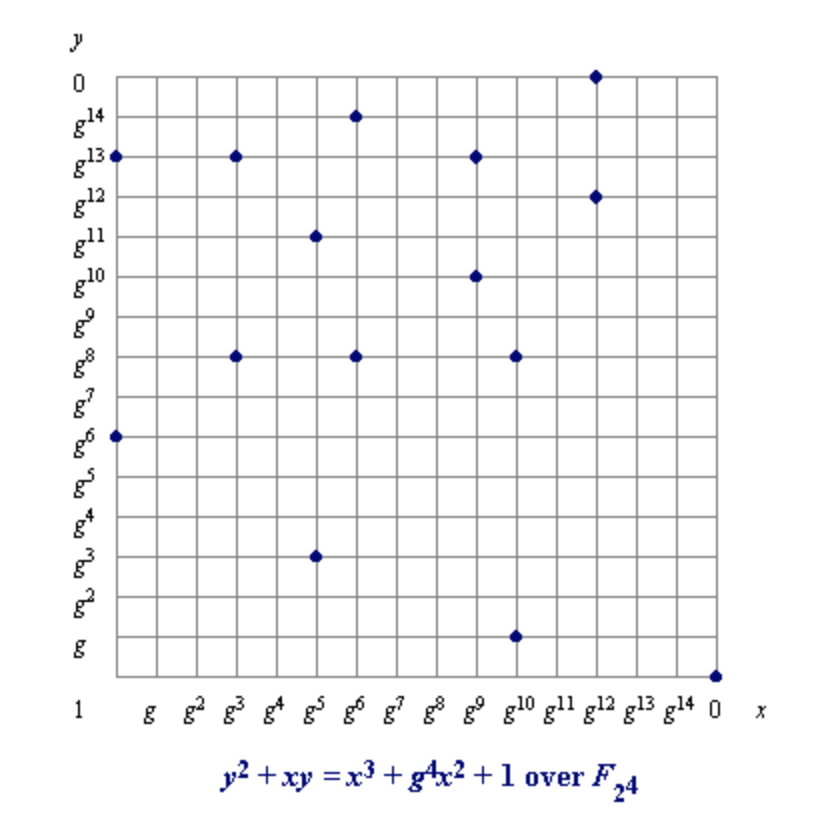
\includegraphics[width=80mm]{./pics/example_of_gf2m.png}
    	\caption{Example of elliptic curve over $\mathbb{F}_{2^4}$ }
    	\label{fig:ecc_gf2m_example}
    \end{figure}
    
\section{Point Arithmetic}
\subsection{Point Addition}
Let $P$ and $Q$ be two distinct points on an elliptic curve, and the $P$ is not $-Q$. To add the points $P$ and $Q$, a line \footnote{line is set of points which satisfy the equation $Ax+By+C = 0$ where $A,B,C \in \mathbb{F}_p$} is drawn through the two points. This line will have exactly one additional intersection points with the elliptic curve, which we call $-R$. The point $-R$ is reflected in the x-axis to obtain point R. The law for point addition in an elliptic curve group is $P+Q=R$. Given an example of geometrical graph in figure \ref{fig:ecc_point_addition} \\
    \begin{figure}[h!]
    	\centering
    	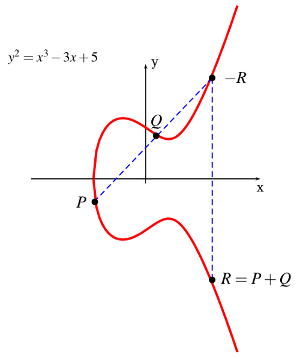
\includegraphics[width=65mm]{./pics/ecc_point_addition.png}
    	\caption{Elliptic curve point addition}
    	\label{fig:ecc_point_addition}
    \end{figure}
    
For point addition of $P$ and $-P$, the line through $P$ and $-P$ is a vertical line which does not intersect the elliptic curve at a third point. Thus the point $P$ and $-P$ can not be added using the above method. It's for this reason that the elliptic curve group includes point $O$, the point at infinity and it is defined as $P + (-P) = O$. 

\subsection{Point Doubling}
Adding a point $P(x,y)$ to itself, a so called tangent line to the curve is drawn at point $P$. If y is not zero, then the tangent line has exact one intersection with the curve at point $-Q$. $-Q$ is reflected in the x-axis to point $Q$. This operation is called doubling the point $P$, and the law for doubling is the following and also shown in figure \ref{fig:ecc_point_doubling}: 
$$P+P=2P=Q$$ 

    \begin{figure}[h!]
    	\centering
    	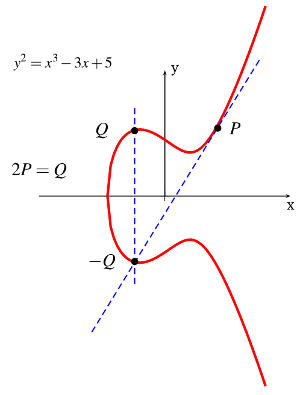
\includegraphics[width=65mm]{./pics/ecc_point_doubling.png}
    	\caption{Elliptic curve point doubling}
    	\label{fig:ecc_point_doubling}
    \end{figure}
    
Doubling the point $P(x,y)$ while $ y=0 $ then the tangent line to the elliptic curve is vertical and does not intersect the elliptic curve on any other points. For such a $P$, by definition, $2P=O$, and $3P$ in this case, is $2P+P = O + P = P$.   

\subsection{Explicit Formulas} \label{sec:affine_formulas}
For elliptic curves over $\mathbb{F}_p$, consider two points $P=(x_1,y_1)$ and $Q=(x_2,y_2)$, $P \neq \pm Q$, the point $P+Q = (x_3,y_3)$ is given by:
$$\lambda = \frac{y_2-y_1}{x_2-x_1}$$
$$x_3=\lambda^2-x_1-x_2$$
$$y_3=\lambda(x_1-x_3)-y_1$$

When $P=-Q$, $P+Q$ equals point at infinity $O$. When $P=Q$, we apply the doubling formula:
$$\lambda = \frac{3x_1^2+a}{2y_1}$$
$$x_3=\lambda^2-2x_1$$
$$y_3=\lambda(x_1-x_3)-y_1$$

For elliptic curves over $\mathbb{F}_{2^m}$, the curve equation $E$ is $$E: y^2+xy=x^3+ax^2+b$$ where $b \neq 0$. Let $P=(x_1,y_1) \in E$; then $-P = (x_1,y_1+x_1)$. If $Q=(x_2,y_2) \in E$ and $Q \neq \pm P$, then $P+Q=(x3,y3)$ is given by:
$$x_3=(\frac{y_1+y_2}{x_1+x_2})^2+\frac{y_1+y_2}{x_1+x_2}+x_1+x_2+a$$
$$y_3=(\frac{y_1+y_2}{x_1+x_2})(x_1+x_3)+x_3+y_1$$
and point doubling for $P=Q$ is given by:
$$x_3=x_1^2+\frac{b}{x_1^2}$$
$$y_3=x_1^2+(x_1+\frac{y_1}{x_1})x_3+x_3$$


\subsection{Point Multiplication and ECDLP}
Given an elliptic curve $E$ defined over a finite field $\mathbb{F}_p$. If $P \in E$ is a point of order r, the cyclic subgroup of $E$ generated by $P$ is ${O,P,2P,\ldots,(r-1)P}$. Then if we define the scalar $k$ as an integer within the range $[1,r-1]$, we can represent point multiplication, also known as scalar multiplication as the following: $Q=kP$, where $Q$ is also a point in the subgroup generated by $P$. 

The hardness of cryptosystem using elliptic curve point multiplication is based on the Elliptic Curve Discrete Logarithm Problem, which is an adaptation of traditional discrete logarithm problem to elliptic curves.

\begin{mydef}
Elliptic Curve Discrete Logarithm Problem (ECDLP) : Given an elliptic curve $E$ defined over a finite field and two points $P,Q \in E$, find an integer $k$ such that $Q = kP$ if such $k$ exists.
\end{mydef}

The ECDLP is assumed to be harder to solve than other recognized problems such as integer factorization and the discrete logarithm problem in the multiplicative group of a finite field, which are the foundations of RSA \cite{rivest1978method} and the ElGamal \cite{elgamal1985public} cryptosystems.``Harder to solve" implies shorter keys are needed to provide same level of security as recommended by \cite{barker2006recommendation}. Table \ref{tab:nist key length} shows the comparison for elliptic curves and RSA.  

\begin{table}[!h]
	\centering
	\caption{NIST's recommendation for key management }
	\label{tab:nist key length}
	\begin{tabular}{|c|c|c|c|c|}
		\hline
		Security level in bits & Block cipher & $\mathbb{F}_p$  & $\mathbb{F}_2^m$ & RSA   \\ \hline
		80                     & SKIPJACK     & 192 & 163 & 1024  \\ \hline
		112                    & Triple-DES   & 224 & 233 & 2048  \\ \hline
		128                    & AES Small    & 256 & 283 & 3072  \\ \hline
		192                    & AES Medium   & 384 & 409 & 7680  \\ \hline
		256                    & AES Large    & 521 & 571 & 15360 \\ \hline
	\end{tabular}
\end{table}
Common methods for solving ECDLP are Pollard’s rho algorithm and index-calculus method, we refer readers to \cite{hankerson2006guide} for more details.
\section{Open Research Questions}
\subsection{Summation Polynomials} \label{sec:summationPoly}
Let $E$ be a general elliptic curve over field $F$ in Weierstrass form given by the equation \ref{eq:ECWeierstrass} we define $$ S_{2}\left( X_1,X_2\right)  = X_1-X_2 \in F\left[ X_1,X_2 \right] $$ The third summation polynomial to be the polynomial $S_{3}\left( X_1,X_2,X_3\right)  \in F \left[ X_1,X_2,X_3\right]$ of degree 4 by  \cite{kosters2015notes}: 
\begin{equation} \label{eq:general_Semaev}
S_{3}\left( X_1,X_2,X_3 \right) =\left( X_1^2X_2^2+X_1^2X_3^2+X_2^2X_3^2\right) - 2\left( X_1^2X_2X_3+X_1X_2^2X_3+X_1X_2X_3^2\right) 
\end{equation}
$\text{\space\space\space\space\space\space\space\space\space\space\space\space\space\space\space\space\space\space\space\space\space\space\space\space\space\space\space\space\space\space\space\space} -d_2\left(X_1X_2X_3 \right) -d_4\left(X_1X_2+X_1X_3+X_2X_3 \right) -d_6\left( X_1+X_2+X_3\right) -d_8$ \\

then for $m \geq 4 $ in any case: \\
$S_m(X_1,\dots,X_m)=\text{Res}_X\left( S_{m-r}\left(X_1,\dots, X_{m-r-1},X \right), S_{r+2}(X_{m-r}\left( X_{m-r},\dots,X_m,X\right)  \right) $\\
where $1 \leq r \leq m-3$.

Summation Polynomials were first introduced by Semaev in 2004 \cite{semaev2004summation}. Semaev's summation polynomials have the property that if $S_m(a_1,\dots,a_m) = 0 $ for some field elements $a_1,\dots,a_m \in F$ if and only if there are elliptic curve points $\left( a_1, b_1\right), \dots,\left( a_m,b_m \right) $ on $E$ such that $\left( a_1, b_1\right)+ \dots + \left( a_m, b_m\right) = 0 $. The idea is to represent point addition in elliptic curves using a multivariate equation system and trying to solve the equation system. This topic has been studied by a lot of researchers trying to solve the ECDLP problem \cite{diem2011discrete,gaudry2004index,faugere2014using,faugere2012improving,petit2012polynomial,huang2013improvement}. In 2015 a new method was introduced by Semaev \cite{cryptoeprint:2015:310} and the idea is trying to solve the equation system by introducing new variables that lower the degree of the system of equations. In this section we will look at Semaev's summation polynomials $S_3\left( X_1,X_2,X_3\right) $ for curves over $\mathbb{F}_p$ and $\mathbb{F}_2^m$, then introduce some open research questions for future work.  \\

\paragraph{Elliptic Curves Over $\mathbb{F}_p$} \mbox{} \\
For an elliptic curve over a field $K$ of characteristic $> 3$ we recall the curve equation \ref{eq:ECFp}
$y^3=x^3+a_4x+a_6$ and $S_3\left( X_1,X_2,X_3\right) $ equation can be simplified to: \cite{kosters2015notes} 

\begin{equation} \label{eq:fpCurveS3}
\begin{split}
S_3( X_1,X_2,X_3) &=( X_1^2X_2^2+X_1^2X_3^2+X_2^2X_3^2)- 2( X_1^2X_2X_3+X_1X_2^2X_3+X_1X_2X_3^2) \\
&\text{\space \space \space } -2a_4(X_1X_2+X_1X_3+X_2X_3 ) -4a_6( X_1+X_2+X_3) +a_4^2 \\
&= ( X_1-X_2)^2X_3^2-2( ( X_1X_2+a_4)(X_1+X_2 ) + 2a_6) X_3 + \left(X_1X_2-a_4 \right) ^2 \\
&\text{\space \space \space } - 4a_6(X_1+X_2)
\end{split}
\end{equation}

and it's also easy to get for point doubling when $X_1=X_2$ we have \\
\begin{equation} \label{eq:fpCurveS3Double}
-2\left( X_1^3 + 2a_4X_1+2a_6\right)X_3+\left( X_1^2 - a_4 \right)^2 - 8a_6X_1 = 0
\end{equation}
\paragraph{Special Curve secp256k1} \mbox{ } \\
For curve secp256k1 \footnote{Elliptic curve used in bitcoin, we will give more details in section \ref{sec:secp256k1} } where $a_4 = 0$ and $a_6 = 7$, equation \ref{eq:fpCurveS3} and equation \ref{eq:fpCurveS3Double} can be written as the following:

\begin{equation} \label{eq:secp256CurveS3}
\begin{split}
S_3( X_1,X_2,X_3) &= ( X_1-X_2)^2X_3^2-2( ( X_1X_2)(X_1+X_2 ) + 14) X_3 + X_1^2X_2^2 \\
&\text{\space \space \space } - 28(X_1+X_2)
\end{split}
\end{equation}
and for point doubling when $X_1=X_2$
$$ -2\left( X_1^3 + 14\right)X_3+ X_1^4 - 56 X_1 = 0 $$
$$ X_3 = \frac{X_1^4-56X_1}{2X_1^3+28}$$

\paragraph{Elliptic Curves Over $\mathbb{F}_{2^m}$} \mbox{} \\
For an elliptic curve over a $\mathbb{F}_2^m$, we have curve equation $y^2+xy=x^3+a_2x^2+a_6$
We have $d_2=1$, $d_4=0$, $d_6=0$ and $d_8=a_6$ (see section \ref{sec:EC}). In binary field anything multiply by 2 equal to 0, $A-B=A+B$, thus equation \ref{eq:general_Semaev} can be simplified to:
$$S_3(X_1,X_2,X_3) = (X_1^2X_2^2+X_1^2X_3^2+X_2^2X_3^2)-X_1X_2X_3-a_6$$
$$\text{\space\space\space\space\space\space\space\space\space\space\space\space\space\space\space\space\space\space\space\space\space\space\space\space\space\space} = \left( X_1X_2+X_1X_3+X_2X_3 \right) ^2 + X_1X_2X_3+a_6$$
$$\text{\space\space\space\space\space\space\space\space\space\space\space\space\space\space\space\space\space\space\space\space\space\space\space\space\space\space} = \left( X_1X_2+X_1X_3+X_2X_3 \right) ^2 + X_1X_2X_3+a_6$$
and when $X_1=X_2$ we have:
$$X_1^4+X_1^2X_3+a_6=0$$
$$X_3=X_1^2+\frac{a_6}{X_1^2}$$

\subsection{Semaev Cipher} \label{sec:SemaevCipher}
In Semaev's recent paper \cite{cryptoeprint:2015:310} he introduced a new algorithm trying to solving ECDLP using summation polynomial for curves over $F_{2^m}$. By recursively compute summation polynomials, instead of trying to write $R=P_1+\cdots+P_m$ for point $P_i$, we can write $Q_1 = P_1+P_2, Q_2=Q_1+P_3, \dots , R = Q_{m-2}+P_m$, where the $Q_i$ are completely arbitrary points (see equation \ref{eq:SemaevCipher}). Then solve the multivariate equation system under some assumptions. 
\begin{equation}
\label{eq:SemaevCipher}
\begin{cases}
S_3(Q_1,P_1,P_2) \cr
S_3(Q_1,Q_2,P_3) \cr
S_3(Q_2,Q_3,P_4) \cr
\vdots \cr
S_3(Q_i,Q_{i+1},P_{i+2}) \cr
\vdots \cr
S_3(Q_{m-2},P_m,R).
\cr
\end{cases}
\end{equation}
However the final result of Semaev's new work is still uncertain, some researchers believes the assumption of Semaev's paper is wrong, cf. later work by Kosters and Yeo \cite{kosters2015notes} and blog posts \cite{StevenECDLP2015,CourtoisECCPost2015}. This leads to some open research questions. 

The new equation system introduced in Semaev's new paper have clear block cipher topology (see figure \ref{fig:blockciphertopology} in section \ref{sec:AA}) \cite{courtois2002cryptanalysis}. It is very similar to the block cipher equations we have tried to solve for GOST and SIMON \cite{courtois2012contradiction,courtois2014combined}. It is potentially to be solved by methods used in algebraic cryptanalysis \cite{courtois2002cryptanalysis}. We call Semaev's new summation polynomial equations \textbf{Semaev cipher} and plan to explore the following research questions:

\begin{enumerate}
	\item Can we solve Semaev cipher using SAT solvers with some clever guessing (similar as our previous work for guess-then-determine attack on GOST)?  
	\item What about the equations when $X_1=X_2$ ? Can we solve those equations efficiently which will lead to speed improvements for the bitcoin elliptic curve implementation?
\end{enumerate}

These questions are not directly related to the password guessing work we are discussing in this part. We will leave it as future work at this moment. 
 
%EC over F_p (point doubling in F_p summation poly)
%cost of dividing by 2 with summation polynomials for bitcoin EC
\subsection{Curves with Special Shortcuts} \label {sec:shortcuts}

Let $E$ be an elliptic curve over $\mathbb{F}_p$ with prime number $p$ and curve order $n$. For any point $Q=(x,y)$ on curve $E$, there exist $\lambda$ and $\zeta$ such that $$\lambda \cdot Q = (\zeta \cdot x , y)$$

So that for computing point multiplication $k \cdot Q$, one can use the above shortcut compute $Q' = \lambda \cdot Q$. Then decompose $k$ to $k=k_1+k_2 \cdot \lambda$ mod $n$. Then $$k \cdot Q = (k_1 + k_2 \cdot \lambda)\cdot Q = k_1\cdot Q + k_2\cdot \lambda \cdot Q = k_1 \cdot Q + k_2 \cdot Q' $$ Since $k_2 \cdot Q'$ can be computed efficiently, total number of point doubling for computing $k\cdot Q$ is reduced. An example have been given for curve secp160k1 in \cite{hankerson2006guide}.

We looked at elliptic curve secp256k1 (used in Bitcoin, detail parameters introduced in section \ref{sec:secp256k1})  where prime $$p= \text{ FFFFFFFF FFFFFFFF FFFFFFFF FFFFFFFF FFFFFFFF FFFFFFFF FFFFFFFE FFFFFC2F}$$ and curve order $$ n = \text{FFFFFFFF FFFFFFFF FFFFFFFF FFFFFFFE BAAEDCE6 AF48A03B BFD25E8C D0364141}$$



For secp256k1, we have $p \equiv 1 \mod{6}$, there exists a primitive 6th root of unity $\zeta \in \mathbb{F}_p$ and  $\zeta^6 - 1 = 0 \mod{n}$. Since $$\zeta^6 - 1 = (\zeta^2-1)\cdot(\zeta^2+\zeta - 1)\cdot (\zeta^2-\zeta -1)$$ 

any root of $\zeta^6-1$ is root of one of the above three polynomials. 

We found special multiples for secp256k1 as following: 

Let
$\lambda_6 =$\\
$AC9C52B33FA3CF1F5AD9E3FD77ED9BA4A880B9FC8EC739C2E0CFC810B51283CF$
%$-5363AD4CC05C30E0A5261C028812645A122E22EA20816678DF02967C1B23BD72$
a primitive 6th root of unity mod $n$.
%==78074008874160198520644763525212887401909906723592317393988542598630163514319
%-37718080363155996902926221483475020450927657555482586988616620542887997980018
%We have $\lambda_6+\lambda_6^2+1=0$ mod $Q$.
We have $\lambda_6-\lambda_6^2-1=0 \mod{n}$.
%mod Q= 115792089237316195423570985008687907852837564279074904382605163141518161494337
%
%\lambda_6^2 = 78074008874160198520644763525212887401909906723592317393988542598630163514318
%=\lambda_6-1
%
%-\lambda_6=37718080363155996902926221483475020450927657555482586988616620542887997980018

Let
$\zeta_6 =$\\
$ 851695D49A83F8EF919BB86153CBCB16630FB68AED0A766A3EC693D68E6AFA40$
be a (not primitive) 6-th root of unity mod $P$.
%a primitive 6-th root of unity mod $P$.
%=60197513588986302554485582024885075108884032450952339817679072026166228089408
%We have $\zeta_6-\zeta_6^2-1$ mod $P$.
We have $\zeta_6+\zeta_6^2+1$ mod $P$.


%mod P=115792089237316195423570985008687907853269984665640564039457584007908834671663
%
%//\zeta_6^2==55594575648329892869085402983802832744385952214688224221778511981742606582254 = 7ae96a2b657c07106e64479eac3434e99cf0497512f58995c1396c28719501eE
%-zeta_6==55594575648329892869085402983802832744385952214688224221778511981742606582255 ==
%7AE96A2B657C07106E64479EAC3434E99CF0497512F58995C1396C28719501EF



We have for ANY point:
$$
\lambda\cdot (x,y) = (\zeta\cdot x,y)
$$

This property is not common for every elliptic curve. We have discovered more special shortcuts like this, and we will investigate how they can be used to speed up the point multiplication process. This should lead to future improvements in the speed of bitcoin ECDSA signature and verification process.

\section{Elliptic Curve Cryptography}
Elliptic curve cryptography (ECC) was independently proposed by Neal Koblitz\cite{koblitz1987elliptic} and Victor Miller in 1985. It is a public-key cryptography protocol where each of the participant has a pair of keys. One private key which is kept as a secret by the owner and one public key which is public potentially for everyone. In the past 10+ years ECC has been increasingly used in practise since its inclusion in standards by organisations such as ISO, IEEE, NIST,etc. Elliptic curves are more efficient \cite{bernstein2009ebacs} and offer smaller key sizes \cite{lenstra2001selecting} at the same security as other widely adopted public key cryptography schemes such as RSA \cite{rivest1978method}. 

There are many widely used elliptic curve cryptographic schemes such as Elliptic Curve Diffie–Hellman (ECDH) key agreement scheme based on the Diffie–Hellman scheme, Elliptic Curve Integrated Encryption Scheme (ECIES), and Elliptic Curve Digital Signature Algorithm (ECDSA) etc. In this part of PhD work we only focus on ECDSA \cite{johnson2001elliptic} (key generation part in particular) which is used in Bitcoin and we refer the readers to \cite{hankerson2006guide} for details of other schemes.

In section \ref{domainParameters} we will describe elliptic curve domain parameters, in section \ref{secKeyPairGen} we will discuss elliptic curve key pair generation process, and briefly introduce ECDSA in section \ref{sec:ecdsa}.

\subsection{Domain Parameters} \label{domainParameters}
Elliptic curve cryptographic schemes need to agree on a fixed elliptic curve and a finite field. The fixed elliptic curves are normally chosen from curves which are suggested by standard organisations, such as ISO, IEEE etc. Different countries might have there own specified standards for choice of elliptic curves, which we will give a list in section \ref{sec:RecomandedCurves}. The specification of a chosen elliptic curve is defined using domain parameters. 

Domain parameters for an elliptic curve scheme describes an elliptic curve $E$ defined over a finite field $\mathbb{F}_p$, a base point $G \in E\left( \mathbb{F}_p \right) $, and its order n. The parameters should be chosen so that the ECDLP is resistant to all known attacks. Domain parameters are defined as the following $D=(q,\text{FR},S,a,b,G,n,h)$ where
\begin{enumerate}
	\item q is the field order
	\item FR (field representation) is an indication of the representation used for the elements of $\mathbb{F}_q$
	\item If the curve is randomly generated, S is the seed used to generated the curve
	\item $a,b \in \mathbb{F}_q$ that define the curve equation over field $\mathbb{F}_q$
	\item $G$ is the base point where $G = \left( G_x,G_y \right) \in E(\mathbb{F}_q)$
	\item The order $n$ of $G$
	\item The cofactor $h = \frac{\#E(\mathbb{F}_q) }{n}$
\end{enumerate}

\subsection{Key Pair Generation}\label{secKeyPairGen}
An elliptic curve key pair is associated on a particular set of valid domain parameters (cf. \cite{hankerson2006guide} for generating and verify EC domain parameters). The public key is a random generated point $Q$ in the group $\left\langle G \right\rangle $ generated by G. The corresponding private key is $d = \log_GQ$. Key pair generation algorithm is the following:
 
\begin{algorithm}[H]
Input: Domain parameters $D=(q,FR,S,a,b,G,n,h)$ \\
Output: Public key $Q$, private key $d$ 
\caption{Key pair generation \cite{hankerson2006guide}}
 \label{al:ECKey_gen}
 \begin{algorithmic} [1]
	\STATE Select $d \in _R \left[ 1, n-1 \right] $.
	\STATE Compute $Q = dP$.
	\STATE Return ($Q,d$).
 \end{algorithmic}
\end{algorithm}
Note that the process of computing a private key $d$ given public key $Q$ is exactly the elliptic curve discrete logarithm problem. Hence it is very import to chose a set of domain parameters so that the ECDLP is hard to solve. In addition the numbers $d$ should be \textbf{random} in the sense that the probability of any particular value being selected must be sufficiently small to avoid an adversary from gaining advantage through optimising a search strategy based on such probability. 

Not all the key pairs are valid keys. A public key $Q=(Q_x,Q_y)$ is valid if it satisfies all the following requirements:
\begin{enumerate}
	\item $Q \neq O$ ( $O$ is the point at infinity)
	\item $Q_x$ and $Q_y$ are properly represented elements of $\mathbb{F}_q$ (i.e., integers in [$0,q-1$] for prime field and bit strings of length m for binary field $\mathbb{F}_2^m$)
	\item $Q$ satisfies the elliptic curve equation defined by $a$ and $b$
	\item $nQ=O$
\end{enumerate}
\subsection{Elliptic Curve Digital Signature Algorithm} \label{sec:ecdsa}
Elliptic Curve Digital Signature Algorithm (ECDSA) is a mathematical scheme based on elliptic curve cryptography that authenticates the identity of a message signer, and checks that the content of the message is not modified. ECDSA is the most widely standardised elliptic curve based signature scheme, appearing in the FIPS 186-2\cite{fips2000186}, IEEE 1363-2000 \cite{ieee2000ieee}, ANSI X9.62 \cite{ansi2005x9} etc. Typically, ECDSA is consists of three parts: key generation, signing and verification. We have discussed the key generation part in previous section, see algorithm \ref{al:ECKey_gen}. Now we look at sign and verification algorithms. 

Let $m$ be the message that the sender want to send, the message sender obtained his EC key pair $d$ and $Q$ using the key generation algorithm using an elliptic curve defined by a set of domain parameters $D=(q,FR,S,a,b,G,n,h)$. The process for signature generation are described in algorithm \ref{alg:ECDSA_sign}. In the following algorithms, $H$ denotes a cryptographic hash function whose outputs have length no more than $n$ (otherwise, the outputs of $H$ can be truncated).

\begin{algorithm}[H] 
	\caption{ECDSA signature generation\cite{hankerson2006guide}}
		Input: Domain parameters $D=(q,FR,S,a,b,G,n,h)$, private key $d$, message $m$ \\
		Output:  Signature ($r,s$)
	\label{alg:ECDSA_sign}
	\begin{algorithmic} [1]
		\STATE Select $k \in _R \left[ 1, n-1 \right] $.
		\STATE Compute $kP=(x_1,y_1)$ and covert $x_1$ to an integer $\bar{x}_1$.
		\STATE Compute $r = \bar{x}_1$ mod $n$. If $r = 0$ then go to step 1.
		\STATE Compute $e = H(m)$.
		\STATE Compute $s = k^{-1}(e+dr)$ mod $n$. If $s=0$ then go to step 1.
		\STATE Return ($r,s$).
	\end{algorithmic}
\end{algorithm}
Anyone can verify the sender signature by using the sender's public key and the process is described as following:
\begin{algorithm}[H] 
	\caption{ECDSA signature verification\cite{hankerson2006guide}}
	Input: Domain parameters $D=(q,FR,S,a,b,G,n,h)$, public key $Q$, message $m$, signature ($r,s$) \\
	Output:  Acceptance or rejection of the signature
	\label{alg:ECDSA_verify}
	\begin{algorithmic} [1]
		\STATE Verify that $r$ and $s$ are integers in the interval $[1,n-1]$. If any verification fails, reject the signature
		\STATE Compute $e = H(m)$.
		\STATE Compute $w=s^{-1}$ mod $n$.
		\STATE Compute $u_1 = ew$ mod $n$ and $u_2=rw$ mod $n$.
		\STATE Compute $X = u_1P+u_2Q$.
		\STATE If $X$ is point at infinity $O$ then reject the signature
		\STATE Covert the $x$-coordinate $x_1$ of X to an integer $\bar{x}_1$; compute $v=\bar{x}_1$ mod $n$.
		\STATE if $v=r$ then accept the signature otherwise reject the signature.
	\end{algorithmic}
\end{algorithm}

\chapter{Bitcoin and Brain Wallet Attacks}

Bitcoin is a virtual currency, an electronic payment system based on cryptography. It was invented by Satoshi Nakomoto\footnote{It's not known whether Satoshi Nakomoto is a real or pseudonym name or if it represents on or a group} in 2008 \cite{nakamoto2008bitcoin}. In 2009, Bitcoin was lunched as an open-source software. Bitcoin is designed to be fully decentralised based on peer-to-peer network, which means self-governing without support from trust entities, banks or government. Bitcoin transactions are like checks but signed cryptographically instead of using ink. Transactions are broadcast to the peer-to-peer network and each node in the peer-to-peer network can verify them. Transactions are recordedin a public distributed ledger called the block chain. All bitcoin transaction history is public and pseudonymous.

Creation of new bitcoins is through a process called mining and participants are called miners. Miners offer their computation power to solve a hard mathematics problem, winners will be rewarded the newly created bitcoin. Chance of winner a reward is directly related to the miner's computation power. During the process of mining, transactions have been processed and recorded into the block chain. 

Ownership of bitcoins implies that a user can spend bitcoins associated with a specific address (equivalent to a bank account). In order to spend the coins, a payer must digitally sign the transaction using their corresponding private key. Then broadcast the signed transaction to the peer-to-peer network. Everyone else in the network can verify the signature that has been send out. Anyone can spend all the bitcoin in a bitcoin address as long as they hold the cosponsoring private key. Once the private is lost, the bitcoin network will not recognize any other evidence of ownership.

Bitcoin uses digital signature protect the ownership bitcoin and private key is the only evidence of owning bitcoin. Thus it is very important to look at the technical details of the digital signature scheme used in bitcoin. In the next section we look at bitcoin brain wallet, our main attack target in this part of research work. We discuss the technical details of how bitcoin address are generated, using which elliptic curve, and how the curve is defined.

\section{Bitcoin Elliptic Curve} \label{sec:secp256k1}
Bitcoin uses elliptic curve digital signature algorithm (see section \ref{sec:ecdsa}). The elliptic curve used in bitcoin is called secp256k1. In the FIPS 186-2 standard \cite{fips2000186} NIST recommends five elliptic curves for use in the curve digital signature algorithm targeting five different security levels (192,224,256,384,521). In the standard, these curves are name P-192, P-224, P-256, P-384, and P521 \footnote{in practice also appear as nistp192, nistp224 etc, in Certicom recommended curves they are named as secp***r1, and in openssl they are called prime***v1}. The bitcoin elliptic curve is proposed in Certicom \cite{certicom2000sec} in addition to NIST curve for 256 bits prime. Secp256k1 is defined over prime field $\mathbb{F}_p$ where the domain parameters $(p,a,b,G,n,h)$ are defined as following:
$$p= \text{ FFFFFFFF FFFFFFFF FFFFFFFF FFFFFFFF FFFFFFFF FFFFFFFF FFFFFFFE FFFFFC2F}$$
$$= 2^{256} - 2^{32} - 2^9 - 2^8 - 2^7 - 2^6 - 2^4 - 1$$
The curve equation $E$ is $y^2 = x^3 + ax +b $ where $a = 0$ and $b = 7$. The base point $G:(G_x,G_y)$ is defined as:
$$G_x = \text{79BE667E F9DCBBAC 55A06295 CE870B07 029BFCDB 2DCE28D9 59F2815B 16F81798}$$
$$G_y = \text{483ADA77 26A3C465 5DA4FBFC 0E1108A8 FD17B448 A6855419 9C47D08F FB10D4B8}$$
and the order n of G and the cofactor h are:
$$ n = \text{FFFFFFFF FFFFFFFF FFFFFFFF FFFFFFFE BAAEDCE6 AF48A03B BFD25E8C D0364141}$$
$ \text{\space\space }h = 1 $
%These curves along others are also recommended by Certicom in the standards for efficient cryptography SEC2 \cite{certicom2000sec} (see more details on recommended curves in Appendix \ref{app:RecommendedCurves}).

\section{Brain Wallet} \label{sec:brainWallet}
Bitcoin wallet is a collection of your bitcoin addresses and stores the corresponding key pairs for those addresses. Bitcoin wallets comes in different form, desktop software, mobile apps, online service, hardware, smart card or paper. The idea it to key your private keys safe. 

As we discussed earlier in section \ref{secKeyPairGen}, the private key is a number which suppose to be totally random. Normally it will be a long hex string which is very hard for a person to remember and stored in your wallet. No matter what form of wallet you are using, there always exist a chance that you might lose your wallet. Even till now, many companies have already provided smart ideas of protecting your private key from hackers, malwares, etc. Users are still required to keep something (maybe not your private key in plain text) safe and hope it won't be stolen in order to recover their private keys once they lost their wallet.    

Brain wallet is another solution, which does not need you to keep anything in safe and still be able to recover you private key. Instead of storing your private key and protecting it, you can store it in your mind. Brain wallet creates private key by a human chosen password or a passphrase, then using SHA-256 hash algorithm to obtain an encrypted hash string. As SHA-256 is deterministic method, you can always use your password remember in your brain to recover the private key. Note that brain wallet uses the hash directly as private key, the security of your private keys now depends on how unpredictable your passwords are. 

Now we give an example show how bitcoin brain wallet are generated by using password ``password"
\begin{enumerate}
	\item Private key: SHA256(``password'') \\ 5E884898DA28047151D0E56F8DC6292773603D0D6AABBDD62A11EF721D1542D8
	\item Public key (uncompressed) : Elliptic curve secp256k1 key pair generation \\ 04B568858A407A8721923B89DF9963D30013639AC690CCE5F555529B77B83CBFC7\\6950F90BE717E38A3ECE1F5558F40179F8C9502DECA11183BB3A3AEA797736A6
	\item SHA256 (Public key) \\
	1D8ED6551EE910136EB0EA735106E137565E8F5EBF8DF73A6A877C92C049F922
	\item Hash160 : RIPEMD160 \\
	3E546D0ACC0DE5AA3D66D7A920900ECBC66C2031\\
	(used for transaction)
\end{enumerate}

 \begin{figure}[h!]
 	\centering
 	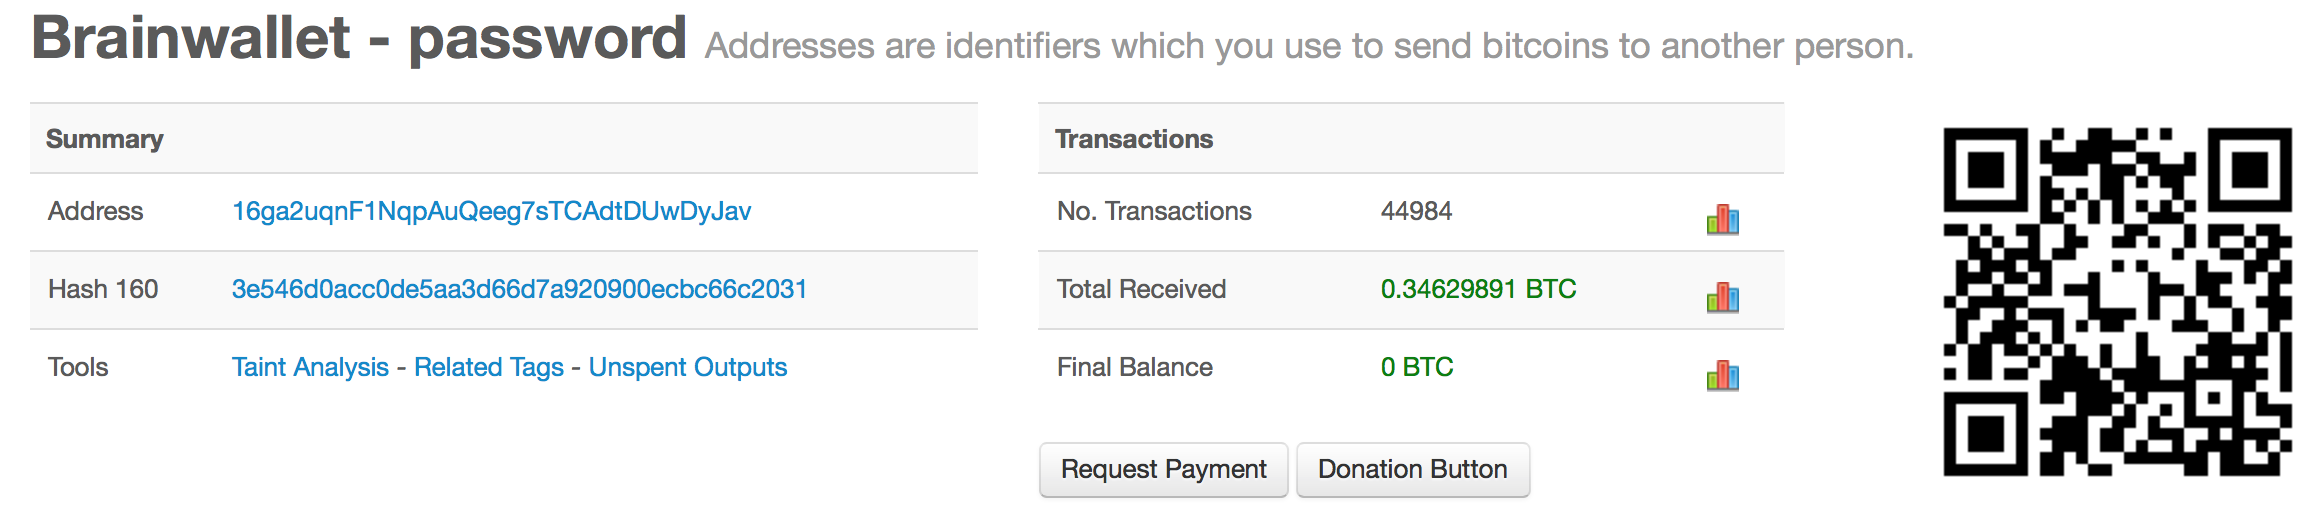
\includegraphics[width=140mm]{./pics/brainwallet-password.png}
 	\caption{Brainwallet generated by password ``password''}
 	\label{fig:brainwallet_password}
 \end{figure}
 
Brainwallet users are normally suggested to use strong password or passphrase. Websites provide brainwallet generation service normally use  figure \ref{fig:password_strength} to tell user what is a strong password. However this figure is a little bit misleading which makes user feels it is safe to use brainwallet with a passphrase. In order to crack brainwallet, there are two directions for optimisation: \textbf{speed} of password guessing and \textbf{efficiency} of password guessing. 

 \begin{figure}[h!]
 	\centering
 	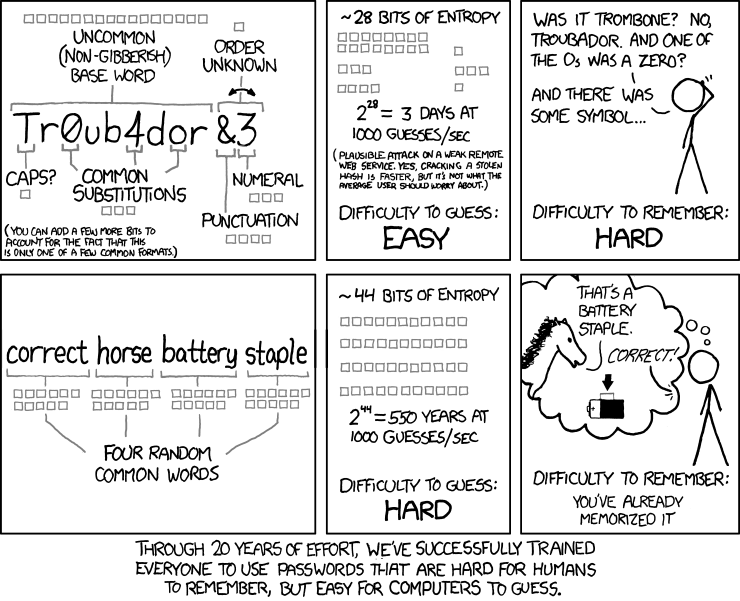
\includegraphics[width=140mm]{./pics/password_strength.png}
 	\caption{password strength comparison between using password and passphrase}
 	\label{fig:password_strength}
 \end{figure}
 
In the next section we will discuss about existing method of bitcoin elliptic curve implementation, benchmarking the state-of-art attack and show an improvement method running the attack with much more faster speed on a laptop. It's also important to note that attacks can use much more CPUs with a cheap price to speed up the password cracking process way more faster.

\section{Bitcoin Elliptic Curve Implementation and Benchmarking}
\subsection{Related Work}
We are not the first one try to crack bitcoin brainwallet, a lot of hackers are doing it. Victims also found their money been stolen and post it in forums. The first brainwallet attack was announced publicly in a recent hacking conference DefCon 23 (Aug 2015). Ryan Castellucci, a white hat hacker presented his attack on cracking brainwallet, and also published his hacking software\cite{RyanDefcon}. Ryan's attack was done on an intel i7 PC with 8 cores. The attack speed can reach approximately 16,250 password per second on each core and he had cracked more than 18,000 brainwallet addresses \footnote{We did contact Ryan in private after his talk and got his detailed results, these numbers are not in his online presentation.}.

The software Ryan has published is using an existing opensource secp256k1 bitcoin elliptic curve implementation mainly written by Pieter Wullie, one of bitcoin core developers. This is considered the current best bitcoin elliptic curve implementation in terms of code level optimisation. Pieter's implementation is written in C based on the Multiple Precision Integers and Rationals (MPIR) library. 

The rest of this section we will look at what has been implemented in Pieter's secp256k1 library, how did the current best attack uses the implementation, show the benckmarking result on our machine, and discuss how did we improved the attack.

\subsection{Special Designed Point Multiplication Method For Attack} \label {sec:specialMethod}
The process of cracking bitcoin brain wallet is to repeatedly generated public keys in bitcoin elliptic curve using generated password. Key generation method as we described in \ref{secKeyPairGen}, is to compute $Q = dP$. Here $d$ is a SHA256 hash of the generated password, $P$ is a fixed point which is the base point $G$ for secp256k1 (see section \ref{sec:secp256k1}). We first benchmark the current best implementation secp256k1 library. All benchmark results are running on a laptop with the following 

\begin{itemize}
	\item CPU: Intel i7-3520m 2.9GHz
	\item RAM: 4G
	\item OS: 64-bit Windows 8
\end{itemize}
The time cost for computing one public key given a random private key takes 
$$\textbf{47.2 us}. $$

\subsubsection{Fixed Point Multiplication Methods}
The most basic and naive method for point multiplication $Q=kP$ with a unknown point $P$ is double-and-add method \cite{hankerson2006guide}.  The idea is to use binary representation for $k$:
$$ k = k_0 + 2k_1 + 2^2k_2+\cdots+2^mk_m$$
where $[k_0\dots k_m]\in \left\lbrace 0,1 \right\rbrace  $ and $m$ is the length of $k$, in bitcoin elliptic curve, $m = 256$. 

 \begin{algorithm}[H] 
 	\caption{double-and-add method for point multiplication of unknown points\cite{hankerson2006guide}}
 	\label{alg:double-and-add}
 	\begin{algorithmic} [1]
 		\STATE $Q := $ infinity
 		\FOR {$i$ from 0 to $m$} 
 		\STATE if $k_i$ = 1 then $Q := Q+P$  (using point addition)
 		\STATE $P:= 2P$ (using point doubling)
 		\ENDFOR
 		\RETURN $Q$
 	\end{algorithmic}
 \end{algorithm}

The expected number of ones in the binary representation of $k$ is approximately $\frac{m}{2}$, so double-and-add method will need $\frac{m}{2} + mD$ computations in total. However, if the point $P$ is fixed and some storage is available, then the point multiplication operation $Q=kP$ can be accelerated by precomputing some data that depends only on $P$. For example if the points $2P, 2^2P, \dots, 2^{m-1}P$ are precomputed, then the double-and-add method (algorithm \ref{alg:double-and-add}) has expected running time $(\frac{m}{2})A$, and all doublings are eliminated.

In \cite{brickell1993fast} the authors introduced a new method for fix point multiplication. The precomputing step store every multiple $2^iP$. Let $(K_{d-1},\dots,K_1,K_0)_{2^w}$ be the base-$2^w$ representation of $k$, where $d = [m/w]$, and let $Q_j = \sum_{i:K_i=j}2^{wi}P$ for each j, $1 \leq j \leq 2^w-1$, Then 

\begin{equation} 
\begin{split}
kP &= \sum_{i=0}^{d_1}K_i(2^{wi}P) = \sum_{j=1}^{2^w-1}(j\sum_{i:K_i=j}2^{wi}P = \sum_{j=1}^{2^w-1}jQ_j\\
&= Q_{2^w-1}+(Q_{2^w-1}+Q_{2^w-2})+\cdots+(Q_{2^w-1}+Q_{2^w-2}+\cdots+Q_1)
\end{split}
\end{equation}


\begin{algorithm}[H] 
	\caption{Fixed-base windowing method for point multiplication\cite{hankerson2006guide}}
	\label{alg:fixed-baseWindow}
	INPUT: Window width $w$, $d = [m/w]$, $k=(K_{d-1},\dots,K_1,K_0)_{2^w}$\\
	OUTPUT: $kP$
	\begin{algorithmic} [1]
		\STATE Precompute $P_i = 2^{wi}P, 0 \leq i \leq d-1$
		\STATE $A \leftarrow \text{infinity}$, $B \leftarrow \text{infinity}$
		\FOR {$j$ from $2^w-1$ downto $1$} 
		\STATE For each $i$ for which $K_i = j$ do: $B \leftarrow B + P_i$
		\STATE $A \leftarrow A+B$
		\ENDFOR
		\RETURN $A$
	\end{algorithmic}
\end{algorithm}

Algorithm \ref{alg:fixed-baseWindow} has expected running time of  $$(2^w+d-3)A$$ 
By reviewing the literature and checking some other existing methods in \cite{hankerson2006guide} we noticed they are all memory friendly implementations which does not take a lot of memory space for precomputation. However, we are working on a different task and aims to repeatedly run point multiplication method for many many times. We have implemented an extreme version of window method which will take much more precomputation space than methods introduced in \cite{hankerson2006guide}. 

In our implementation, the precomputation step will compute $P_j=jP$ where $ 1 \leq j \leq 2^w-1$ then for each $P_j$ we compute $P_{i,j}=2^{wi}P_j$, which will cost $2^w-1$ times more memory space than algorithm \ref{alg:fixed-baseWindow}, but expected running time for each point multiplication will reduce to approximately $(d-1)A$

\begin{algorithm}[H] 
	\caption{Our implementation of windowing method with larger precomputation table}
	\label{alg:newWindow}
	INPUT: Window width $w$, $d = [m/w]$, $k=(K_{d-1},\dots,K_1,K_0)_{2^w}$\\
	OUTPUT: $kP$
	\begin{algorithmic} [1]
		\STATE Precompute $P_{i,j} = 2^{wi}jP, 0 \leq i \leq d-1$ and $ 1 \leq j \leq 2^w-1$
		\STATE $A \leftarrow \text{infinity}$
		\FOR {$i$ from $0$ to $d-1$} 
		\STATE $A \leftarrow A+P_{i,j}$ where $j = K_i$
		\ENDFOR
		\RETURN $A$
	\end{algorithmic}
\end{algorithm}

We have implemented a code that can take any window width $w$ from 1 to 24\footnote{larger than 22 will take too long for precomputation and my laptop start to have slow response}, our benchmark results are shown in table \ref{tb:benchmarkWindowSize1}. Note that precomputation stores elliptic curve point $P = {x,y}$ where $x$ and $y$ are 32 bits integer array of size 10. So one store point need 80 Bytes memory space. 
%\footnote{it will take a long time for my laptop to do precomputation when $w \gt 28$}

\begin{table}[h]
	\centering
	\caption{Time cost for different window width $w$, point addition method secp256k1 library \cite{Wulliesecp256k1} secp256k1\_gej\_add\_ge }
	\label{tb:benchmarkWindowSize1}
	\begin{tabular}{|c|c|c|c|c|c|}
		\hline
		& w=4 & w=8 & w=12 & w=16 & w=20 \\ \hline
		d         & 64  & 32  &  22  & 16   &   13   \\ \hline
		number of additions & 63 & 31 & 21 & 15 & 12 \\ \hline
		precomputation memory & 81.92 KB & 655.36 KB & 7.21 MB & 83.89 MB & 1.09 GB \\ \hline 
		time cost &  46.36 us & 22.76 us  &  15.35 us & 11.23 us &  9.23 us \\ \hline
	\end{tabular}
\end{table}
\subsection{Point Representation} \label{sec:pointRep}
As we described in section \ref{sec:affine_formulas}, representing a point in affine coordinate $P(x,y)$ on an elliptic curve over $\mathbb{F}_p$, the field operations for calculating point addition need 2 multiplications, 1 square and one modular inverse (for short, 2M+1S+1I). Modular inverse is more expensive operation compare to multiplication and square. We list our benchmarks using different package in C to demonstrate the difference for modular inverse computation compare to multiplication and square. The packages we are benchmarking are: openssl-1.0.2a (released in March 2015) and mpir-2.5.2 (released in Oct 2012), and the Pieter Wullie's implementation on github \cite{Wulliesecp256k1} \footnote{with the following configuration: USE\_NUM\_GMP USE\_FIELD\_10x26 USE\_FIELD\_INV\_NUM USE\_SCALAR\_8x32 USE\_SCALAR\_INV\_BUILTIN} . 


 The results are shown in table \ref{table:benchmark_msi_affine}. The benchmarking shows modular inverse is much more expensive than multiplication and square. It is also important to notice, for openssl big number library, square operation is more expensive than multiplication, and for MPIR library, 1 square = 0.75 multiplication. As modular inverse is expensive than multiplication, it may be advantageous to represent points using other coordinates.
 
 \begin{table}[]
 	\centering
 	\caption{Benchmarking openssl and MPIR library for field multiplication, square and modular inverse in affine coordinate}
 	\label{table:benchmark_msi_affine}
 	\begin{tabular}{|c|c|c|c|c|c|}
 		\hline
 		& multiplication     & mod p    & square         & mod p        & mod inverse \\ \hline
 		MPIR      & 0.07 us            & 0.15 us    & 0.13 us        & 0.15 us        & 18.0 us     \\ \hline
 		openssl   & 0.08 us            & 0.43 us    & 0.06 us        & 0.43 us        & 1.8 us      \\ \hline
 		secp256k1 & \multicolumn{2}{c|}{0.049 us} & \multicolumn{2}{c|}{0.039 us} & 1.1 us      \\ \hline
 	\end{tabular}
 \end{table}

\paragraph{Projective Coordinates} \mbox{}\\
For elliptic curve over $\mathbb{F}_p$ where the curve equation is $y^2=x^3+ax+b$. The standard projective coordinates represent elliptic curve points as ($X:Y:Z$), $Z \neq 0$, correspond to the affine point ($\frac{X}{Z},\frac{Y}{Z})$. The projective equation of the elliptic curve is: $$Y^2Z=X^3+aXZ^2+bZ^3$$ The point at infinity $O$ corresponds to (0:1:0), where the negative of ($X:Y:Z$) is $(X:-Y:Z)$ 
\paragraph{Jacobian Coordinates} \mbox{}\\
Elliptic curve points in Jacobian coordinate are represented in the following format ($X:Y:Z$), $Z \neq 0$, corresponds to the affine point $(\frac{X}{Z^2},\frac{X}{Z^3})$. The projective equation of the elliptic curve is $$ Y^2=X^3+aXZ^4+bZ^6$$ The point at infinity $O$ corresponds to (1:1:0), while the negative of ($X:Y:Z$) is ($X:-Y:Z)$.
 
The field operations need for point addition and point doubling are shown in table \ref{tb:APJacobian}. We see that Jacobian coordinates yield the fastest point doubling, while mixed Jacobian-affine coordinates yield the fastest point addition.

\begin{table}[h]
	\centering
	\caption{Operation counts for point addition and doubling. A = affine, P = standard projective, J = Jacobian \cite{hankerson2006guide,brown2001software}}
	\label{tb:APJacobian}
	\begin{tabular}{|cc|cc|ll|}
		\hline
		\multicolumn{2}{|c|}{Doubling} & \multicolumn{2}{c|}{General addition} & \multicolumn{2}{c|}{Mixed coordinates*} \\ \hline
		2A $\rightarrow$ A         & 1I,2M,2S        & A+A $\rightarrow$ A            & 1I,2M,1S           & \multicolumn{1}{c}{J+A $\rightarrow$ J}    & 8M,3S   \\
		2P $\rightarrow$ P         & 7M,3S           & P+P $\rightarrow$ P            & 12M,2S             &                              &         \\
		2J $\rightarrow$ J         & 4M,4S           & J+J $\rightarrow$ J            & 12M,4S             &                              &         \\ \hline
	\end{tabular} \par
	\bigskip
	* Here mixed coordinates means Jacobian-Affine mixed coordinates, see below for details.
\end{table}

We refer the reader to \cite{hankerson2006guide,brown2001software} for other detailed equations in different coordinates. Here we only interested in point addition functions using mixed coordinates. 

\paragraph{Point Addition using Jacobian-Affine Mixed Coordinates} \mbox{} \\
Let $P = (X_1:Y_1:Z_1)$ be a Jacobian projective point on elliptic curve $y^2=x^3+ax+b$, and $Q = (X_2:Y_2:1)$ be be another point on the curve, suppose that $P \neq \pm Q$, $P+Q=(X_3:Y_3:Z_3)$ is computed by the following equations:
\begin{equation} \label{eq:8m3s}
\begin{split}
X_3 = &(Y_2Z_1^3-Y_1)^2 - (X_2Z_1^2-X_1)^2(X_1+X_2Z_1^2) \\
Y_3 = &(Y_2Z_1^3-Y_1)(X_1(X_2Z_1^2-X_1)^2-X_3)-Y_1(X_2Z_1^2-X_1)^3 \\
Z_3 = &(X_2Z_1^2-X_1)Z_1 
\end{split}
\end{equation}

By storing the intermediate elements, $X_3,Y_3$ and $Z_3$ can be computed using three field squarings and eight field multiplications as follows:
$$ A \leftarrow Z_1^2, \text{ } B \leftarrow Z_1 \cdot A,  \text{ } C \leftarrow X_2 \cdot A,  \text{ } D \leftarrow Y_2 \cdot B,  \text{ }  E \leftarrow C - X_1,$$
$$ F \leftarrow D - Y_1, \text{ } G \leftarrow E^2, \text{ } H \leftarrow G \cdot E, \text{ } I \leftarrow X_1 \cdot G, $$
$$ X_3 \leftarrow F^2 - (H+2I), \text{ } Y_3 \leftarrow F \cdot (I - X_3) - Y_1 \cdot H, \text{ } Z_3 \leftarrow Z_1 \cdot E.$$

In \cite{bernstein2007explicit} 

\paragraph{secp256k1 point addition formulas}
In the latest version, secp256k1 point addition formulas are based on \cite{brier2002weierstrass} which introduced a strongly unified addition formulas for standard projective coordinate. Bitcoin developers implemented mixed coordinate formula (Jacobian-Affine) version based on \cite{brier2002weierstrass}. 

Let $P = (X_1:Y_1:Z_1)$ be a Jacobian projective point on elliptic curve $y^2=x^3+ax+b$, and $Q = (X_2:Y_2:1)$ be be another point on the curve, suppose that $P \neq \pm Q$, $P+Q=(X_3:Y_3:Z_3)$ is computed by the following equations:
\begin{equation} \label{eq:7m5s}
\begin{split}
X_3 &= 4 (K^2 - H) \\
Y_3 &= 4 (R(3H-2K^2)-G^2) \\
Z_3 &= 2 F  Z_1
\end{split}
\end{equation}

where
$$ A = Z_1^2, \text{ } B = Z_1 \cdot A, \text{ } C = X_2 \cdot A, \text{ } D = Y_2 \cdot B, \text{ } E = X_1 + C $$
$$ F = Y_1 + D, G = F^2, H = E  \cdot G, I = E^2, J = X_1 \cdot C, K = I - J $$

\paragraph{Bernstein-Lange point addition formulas}
In \cite{bernstein2007faster}, Bernstein introduced the following method which take 7M+4S, the explicit formulas are given as following \cite{bernstein2007explicit}
\begin{equation} \label{eq:7m4s}
\begin{split}
& X_3 = r^2 - J - 2 V \\
& Y_3 = r \cdot (V-X_3)-2Y_1 \cdot J \\
& Z_3 = (Z_1+H)^2 - Z_1^2 - H^2 \\
\end{split}
\end{equation}
\text{where}\\
\begin{equation*}
\begin{split}
& U2 = X_2 \cdot Z_1^2,\text{ } S2 = Y_2 \cdot Z_1^3 \\
& H = U2 - X_1 , \text{ } I = 4 H^2 \\
& J = H \cdot I , \text{ } r = 2  (S2-Y_1) , \text{ } V = X_1 \cdot I 
\end{split}
\end{equation*}



\paragraph{Detailed Filed Operation Benchmarks} \mbox{} \\
From the results of table \ref {table:benchmark_msi_affine} we saw that Wullie's secp256k1 library \cite{Wulliesecp256k1} have a much faster field multiplication and square speed than openssl and mpir library.
Wullie's field implementation is optimised based on the prime used in secp256k1 curve. Secp256k1 library has 5x52 and 10x26 field implementation for 64 bits and 32 bits integers \footnote {Depends on whether compiler support 64 bits integer}. Here we use 10x26 representation and each 256 bits value is represented as a 32 bits integer array with size of 10. We refer readers to file \textit{field\_10x26\_impl.h} in secp256k1 library for more details. Secp256k1 library already implemented equation \ref{eq:7m5s} in method \textit{secp256k1\_gej\_add\_ge\_var}, which uses 8 multiplications, 3 squares and 12 multiply integer / addition / negation. Equation \ref{eq:8m3s} is implemented in \textit{secp256k1\_gej\_add\_ge} which uses 7 multiplications, 5 squares and 21 multiply integer / addition / negation. We have implemented equation \ref{eq:7m4s} which take 7 multiplication, 4 squares and 22 multiply integer / addition / negation.

It is important to notice the square and multiplication difference we discussed in table \ref{table:benchmark_msi_affine}. In \cite{explicitBernstein} Bernstein listed best operation counts based on different assumptions: S = 0M, S = 0.2M, S= 0.67M, S=0.8M and S=1M. In \cite{cohen1998efficient}, the author discussed the ratio $S/M$ is almost independent of the field of definition and of the implementation, and can be reasonably taken equal to 0.8. Our benchmark results is very similar to S = 0.8M (see table \ref{table:benchmark_msi_affine}). In \cite{bernstein2007explicit}, other field operations are considered as 0M,  in table \ref{tb:fieldoperationcounts} our benchmark results shows field addition and other operations have approximately 0.1M cost. 

\begin{table}[h]
	\centering
	\caption{Field operation counts and benchmark results}
	\label{tb:fieldoperationcounts}
	\begin{tabular}{|c|c|c|c|c|c|}
		\hline
		& \#Multiplication & \#Square & \#add/neg/*int & \#fe\_cmov & total time cost    \\ 
	    & 1M & $\approx$ 0.8 M & $\approx$ 0.1 M  & $\approx$ 0.2 M  &    \\ \hline
		secp256k1\_gej\_add\_ge      & 7                & 5        & 15                 & 6        & $\approx$ 0.681 us \\ \hline
		secp256k1\_gej\_add\_ge\_var & 8                & 3        & 12                 & 0        & $\approx$ 0.562 us \\ \hline
		7M + 4S  code    & 7                & 4        & 21                 & 0        & $\approx$ 0.594 us \\ \hline
	\end{tabular}
\end{table}

The secp256k1\_gej\_add\_ge method which is also the default method for key generation, uses 6 secp256k1\_fe\_cmov operations which has a cost approximately 0.2 M. The main reason of writing code in such a way is stated in the code, the author's comments: \\ \mbox{ } \\
\textit{"This formula has the benefit of being the same for both addition of distinct points and doubling"\cite{Wulliesecp256k1}} \\ \mbox{ } \\ 

The propose of make addition and double using the same function is to prevent side channel attacks. As point doubling is much more cheaper than point addition. Our experiments are done based on the benchmark results of S/M ratio with specified machine setting (earlier in section \ref{sec:specialMethod}) and specific library configuration (footnote in section \ref{sec:pointRep}). Different operating systems or library configurations might have different results. One should choose between our code and secp256k1\_gej\_add\_ge method. Detailed benchmark results are given in table \ref{tb:benchmarkWindowSize}
% Our implementation method is chosen based on the benchmark results. One should chose the best method based on there square and multiplication performance. 

\begin{table}[h!]
	\centering
	\caption{Time cost for different window width $w$ for EC key generation}
	\label{tb:benchmarkWindowSize}
	\begin{tabular}{|c|c|c|c|c|c|}
		\hline
		& w=4                  & w=8       & w=12     & w=16     & w=20               \\ \hline
		d                                                                                                        & 64                   & 32        & 22       & 16       & 13                 \\ \hline
		number of additions                                                                                      & 63                   & 31        & 21       & 15       & 12                 \\ \hline
		precomputation memory                                                                                    & 81.92 KB             & 655.36 KB & 7.21 MB  & 83.89 MB & 1.09 GB            \\ \hline
		secp256k1\_gej\_add\_ge                                                                                  & 45.85 us             & 22.16 us  & 15.35 us & 11.23 us & 9.23 us            \\ \hline
		secp256k1\_gej\_add\_ge\_var                                                                             & \textbf{37.37 us}* & 17.86 us  & 12.21 us & 8.89 us  & \textbf{7.16 us} \\ \hline
		7M + 4S code                                                                                             & 39.01 us             & 18.79 us  & 12.77 us & 9.23 us  & 7.48 us            \\ \hline
		\multicolumn{1}{|l|}{covert Jacobian to Affine}                                                          & \multicolumn{5}{l|}{  $\approx$ 10 us}                                               \\ \hline
		\multicolumn{1}{|l|}{\begin{tabular}[c]{@{}l@{}}Benchmark on my laptop \\ i7-3520m 2.9 GHz CPU\end{tabular}}      & \multicolumn{5}{l|}{$\approx$ 42 K guesses / sec (single thread)}                                  \\ \hline
		\multicolumn{1}{|l|}{\begin{tabular}[c]{@{}l@{}}Defcon Attack**\\ i7-2600 3.2 GHz CPU\end{tabular}}      & \multicolumn{5}{l|}{$\approx$ 130 K guesses / sec}                                  \\ \hline
		\multicolumn{1}{|l|}{\begin{tabular}[c]{@{}l@{}}Improved Defcon attack**\end{tabular}} & \multicolumn{5}{l|}{ $\approx$ 315 K guesses / sec}                                  \\ \hline
	\end{tabular}
	\\ \mbox{} \\ * Defcon attack \cite{RyanDefcon} is equivalent to this results 
	\\ ** Results are reported by Ryan Castellucci running his Defcon code and our improved code on 8 threads with linux gcc compiler.
\end{table}

Defcon attack \cite{RyanDefcon} published code on github in Aug using a faster version of secp256k1 library \footnote{Also written by Pieter Wullie one year ago, this version is performance focused and using 8M+3S}, and the results is marked as * in table \ref{tb:benchmarkWindowSize}.  Our best result using 1.09 GB precomputation memory gives  \textbf{$\approx$ 2.5 times speed up} for key generation process than the current known best attack.

\section{Experiment Results}
We have collected all hash160 on blockchain data (until June 2015), 89,872,723 unique addresses has ever been used, we have cracked 18,250 addresses in total. This is still on going research. I'll show some interesting results during the viva.
\subsection{Network Stress Test}
Currently the maximum block size is one megabyte per block. On 11 November 2014, when the block is around 30\% full, David Hunduson wrote a blog post analyzing what will happen on the network as we approach 100\% full blocks. David Hunduson did a simulation which shows if the block is 100\% full then 10\% of all transactions would still not have received a confirmation after 22800 seconds (6.3 hours).

Later on 4th May, head Bitcoin developer Gavin Andersen discussed this problem in his blog and few days later he suggested to increase the maximum block size to 20MB. Over the past few months, the Bitcoin community has been roiling with a debate about whether or not to implement a code change that would enable Bitcoin to handle worldwide adoption by increasing the size of the blocks on the chain. The catch is that it would split the blockchain in the process, requiring everyone to move over to a new version of the ledger.

As a result of this debate, CoinWallet.eu, a Bitcoin exchange in UK decided to launch a stress test for the Bitcoin network. CoinWallet lunched two stress test 

\subsection{Disclosure of results}
This is still under discussion. All the addresses are currently empty, but some addresses are still in used quite recently. One of the ideas we currently have in mind is to tag the cracked addresses on blockchain.info. See figure \ref{fig:tag_page} and \ref{fig:tagged_address}. But the process is not automated due to captcha requirement and we do have a lot of cracked password.

 \begin{figure}[h!]
 	\centering
 	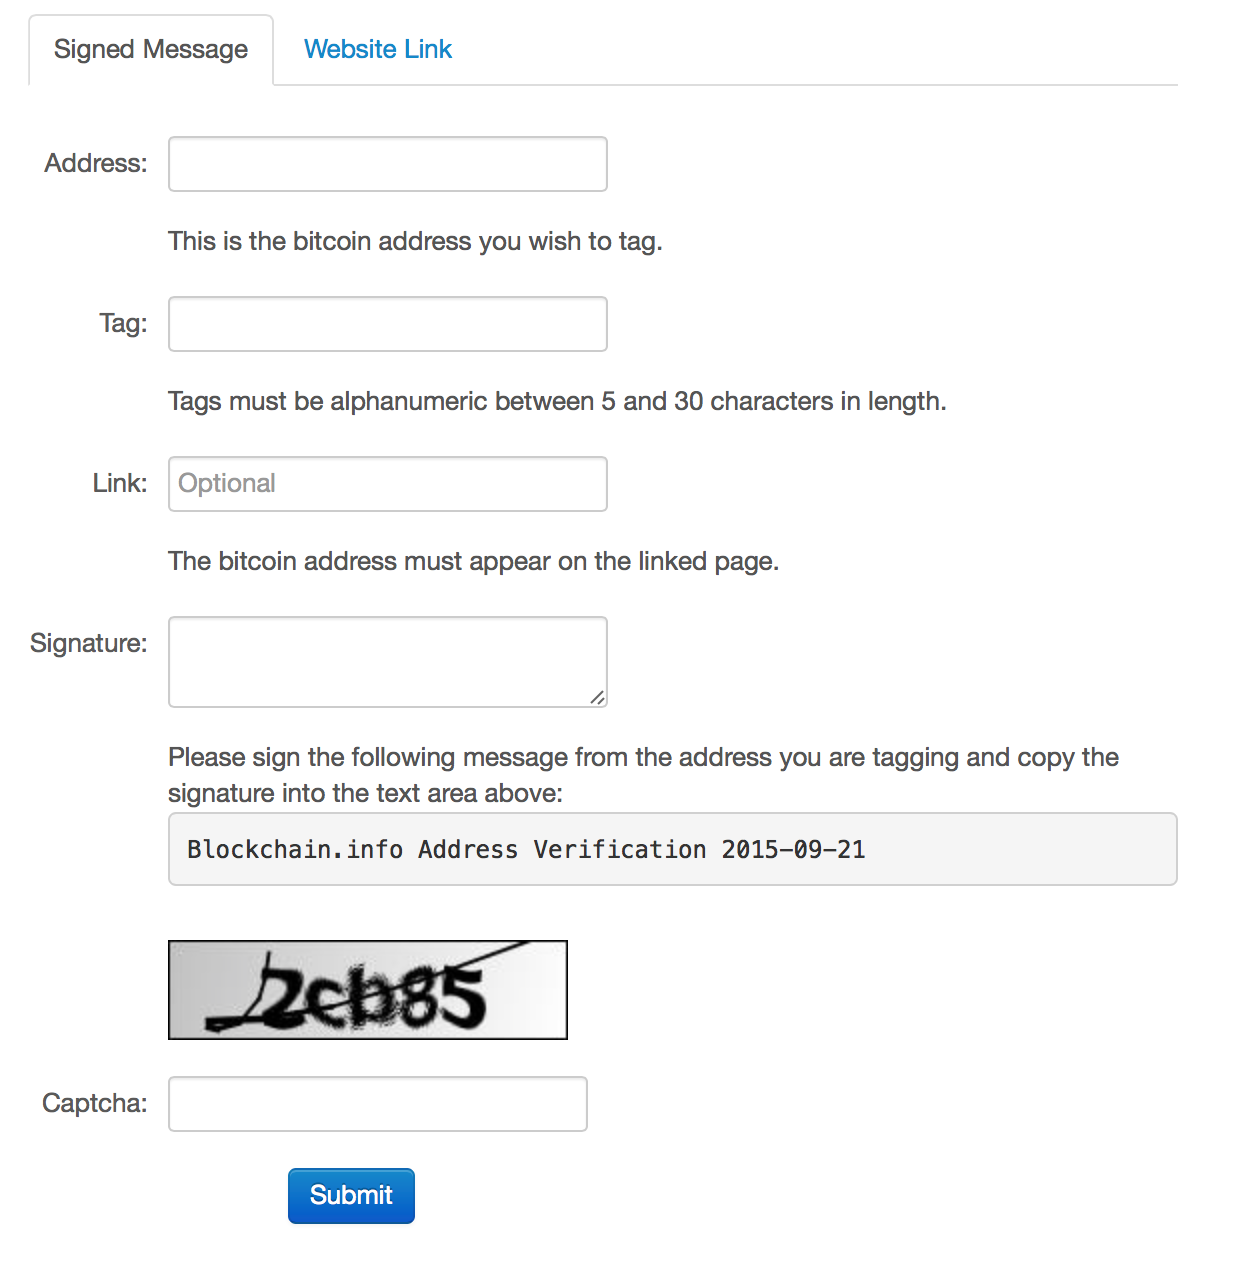
\includegraphics[width=80mm]{./pics/tag_page.png}
 	\caption{Blockchain.info tag address page}
 	\label{fig:tag_page}
 \end{figure}
 
  \begin{figure}[h!]
  	\centering
  	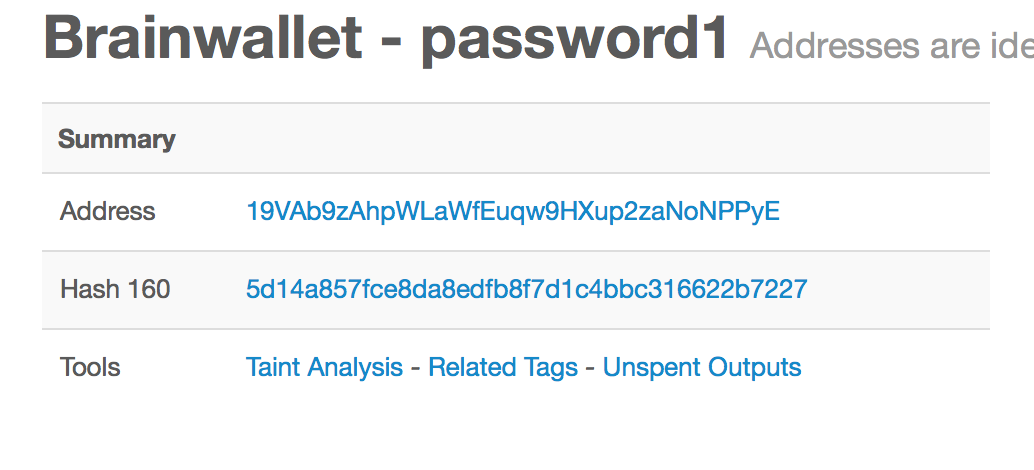
\includegraphics[width=80mm]{./pics/tag_address.png}
  	\caption{Example of tagged brainwallet address }
  	\label{fig:tagged_address}
  \end{figure}

